\chapter{共轭羰基化合物：迈克尔与罗宾逊}\label{ch:b2:conjugate-additions}

甾体激素的四个环最初是逐个组装起来的，其中一类反应
序列成为增加一个环的标准方法：它构建出一个完整的六元环，包括酮基，
由一个酮和一个小的不饱和酮出发。该方法之所以有效，是因为羰基与
\ce{C=C} 双键共轭后，把亲电性传递给该双键的远端。
本章讨论的正是这一远端：哪些亲核试剂进攻它、为什么进攻，以及能用它构建什么。

\begin{recall}
\Cref{ch:b2:enolates-aldol}：\omterm{def:b2:enolates-aldol:enolate}{烯醇负离子}、\omterm{def:b2:enolates-aldol:aldol}{羟醛缩合}。\Cref{ch:b2:frontier-orbitals}：\omterm{def:b2:frontier-orbitals:control}{电荷
控制}与\omterm{def:b2:frontier-orbitals:control}{轨道控制}，硬试剂与软试剂。\Cref{ch:b2:huckel}：休克尔轨道与 $\pi$ 电荷。
本科一年级分册：格氏试剂和氢化物、动力学控制和热力学控制、共轭
体系。
\end{recall}

\section{两个亲电位点}

\begin{definition}[$\alpha,\beta$-不饱和羰基化合物]\label{def:b2:conjugate-additions:enone}
称\emph{$\alpha,\beta$-不饱和羰基化合物}\index{$\alpha,\beta$-不饱和羰基化合物}为
羰基化合物中 $\alpha$ 与 $\beta$ 碳之间有 \ce{C=C} 双键、
且与 \ce{C=O} 共轭的化合物，包括烯酮、烯醛、不饱和酯和腈。
最简单的是丙烯醛 \ce{CH2=CHCHO} 和
丁-3-烯-2-酮 \ce{CH2=CHCOCH3}（甲基乙烯基酮）。
\end{definition}

\begin{omfigure}
\setchemfig{atom sep=1.9em}
\schemestart
\chemfig{H_2C=CH-CH=O}
\arrow{<->}
\chemfig{H_2C=CH-\chemabove{C}{\scriptstyle +}H-\chemabove{O}{\scriptstyle -}}
\arrow{<->}
\chemfig{\chemabove{C}{\scriptstyle +}H_2-CH=CH-\chemabove{O}{\scriptstyle -}}
\schemestop
\par\medskip

\begin{tikzpicture}
\begin{axis}[ybar, width=0.47\linewidth, height=4.6cm, ymin=-0.6, ymax=0.4,
  xtick={1,2,3,4}, xticklabels={C$\beta$,C$\alpha$,C(O),O}, axis x line=bottom, axis y line=left,
  extra y ticks={0}, extra y tick style={grid=major, grid style={black!50}}, enlarge x limits=0.15,
  tick label style={font=\scriptsize}, ylabel={$\pi$ 电荷}, label style={font=\small},
  title={\small 丙烯醛的 $\pi$ 电荷}, bar width=8pt]
\addplot[fill=omDef!50, draw=omDef] table[x=atom, y=q] {figdata/out/bachelor-2-huckel-d.dat};
\end{axis}
\end{tikzpicture}\hfill
\begin{tikzpicture}
\begin{axis}[ybar, width=0.47\linewidth, height=4.6cm, ymin=-0.8, ymax=0.8,
  xtick={1,2,3,4}, xticklabels={C$\beta$,C$\alpha$,C(O),O}, axis x line=bottom, axis y line=left,
  extra y ticks={0}, extra y tick style={grid=major, grid style={black!50}}, enlarge x limits=0.15,
  tick label style={font=\scriptsize}, ylabel={系数}, label style={font=\small},
  title={\small 丙烯醛的 LUMO}, bar width=8pt]
\addplot[fill=omThm!45, draw=omThm] table[x=atom, y=c] {figdata/out/bachelor-2-huckel-d.dat};
\end{axis}
\end{tikzpicture}

{\small 丙烯醛。上：其三种共振结构；后两种使羰基碳与
$\beta$ 碳带正电荷。下：\cref{ch:b2:frontier-orbitals}中的休克尔模型
（$\alpha_{\ce{O}} = \alpha + \beta$，$\beta_{\ce{CO}} = \beta$；仅为模型）。
最大正电荷位于羰基碳上（+0.33，$\beta$ 碳上为 +0.23）；
\omterm{def:b2:frontier-orbitals:frontier}{LUMO} 系数最大处在 $\beta$ 碳上（0.66，相比之下为 $-0.58$）。}
\end{omfigure}

\begin{proposition}[两个位点]\label{prop:b2:conjugate-additions:two-sites}
在 $\alpha,\beta$-不饱和羰基化合物中，羰基碳与 $\beta$ 碳均是
亲电位点。羰基碳带有较大的正电荷；$\beta$ 碳在
\omterm{def:b2:frontier-orbitals:frontier}{LUMO} 中的系数较大。
\end{proposition}

\begin{proof}[论证]
共振结构使羰基碳带正电荷，并通过 \ce{C=C} 使
$\beta$ 碳带正电荷；$\alpha$ 碳从不带正电。丙烯醛的休克尔模型对此作了定量
说明：把 $2c^2$ 对两个占据的 $\pi$ 轨道求和，得到 $\pi$ 电荷
（\cref{def:b2:huckel:indices}）：$+0.33$ 在羰基碳上，$+0.23$ 在 $\beta$ 碳上，$-0.03$
在 $\alpha$ 碳上，$-0.53$ 在氧上。\omterm{def:b2:frontier-orbitals:frontier}{LUMO} 即接收亲核试剂电子的
轨道，其在 $\beta$ 碳上最大。因此两个位点分别对应
\cref{def:b2:frontier-orbitals:control}中的两类控制。
% figdata: bachelor-2/huckel.py part d
\end{proof}

\section{1,2-加成还是共轭加成}

\begin{definition}[加成方式]\label{def:b2:conjugate-additions:addition-modes}
亲核试剂加到 $\alpha,\beta$-不饱和羰基化合物的羰基碳上，得到
\emph{1,2-加成}\index{1,2-加成}（从氧原子起计数）：先生成烯丙基醇盐，再
得到醇。加到 $\beta$ 碳上的亲核试剂得到\emph{共轭加成}\index{共轭加成}
（或 1,4-加成）：生成\omterm{def:b2:enolates-aldol:enolate}{烯醇负离子}，它在碳上被质子化，
得到在 $\beta$ 碳上取代的饱和羰基化合物。
\end{definition}

\begin{omfigure}
\setchemfig{atom sep=1.9em}
\schemestart
\chemfig{*6(-=-(=O)---)}
\arrow{->[\ce{CH3Li}][然后 \ce{H2O}]}[,1.4]
\chemfig{*6(-=-(-[:75]CH_3)(-[:-15]OH)---)}
\schemestop
\hspace{2.5em}
\schemestart
\chemfig{*6(-=-(=O)---)}
\arrow{->[\ce{(CH3)2CuLi}][然后 \ce{H2O}]}[,1.6]
\chemfig{*6(-(-CH_3)--(=O)---)}
\schemestop
\par\vspace{6pt}

{\small 环己-2-烯-1-酮与两种甲基亲核试剂的反应。甲基锂为\omterm{def:b2:frontier-orbitals:hard-soft}{硬亲核试剂}，加到
羰基碳上，得到 1-甲基环己-2-烯-1-醇（\omterm{def:b2:conjugate-additions:addition-modes}{1,2-加成}）。二甲基铜锂为\omterm{def:b2:frontier-orbitals:hard-soft}{软亲核试剂}，
加到 $\beta$ 碳上，得到 3-甲基环己酮（\omterm{def:b2:conjugate-additions:addition-modes}{共轭加成}）。}
\end{omfigure}

\begin{proposition}[加成位点]\label{prop:b2:conjugate-additions:regio}
\omterm{def:b2:frontier-orbitals:hard-soft}{硬亲核试剂}（有机锂试剂、多数格氏试剂、\ce{LiAlH4}）主要进行
\omterm{def:b2:conjugate-additions:addition-modes}{1,2-加成}，受\omterm{def:b2:frontier-orbitals:control}{电荷控制}，通常不可逆。\omterm{def:b2:frontier-orbitals:hard-soft}{软亲核试剂}（\omterm{def:b2:conjugate-additions:cuprate}{有机铜锂试剂}、稳定的\omterm{def:b2:enolates-aldol:enolate}{烯醇负离子}、硫醇盐、
胺）主要进行 1,4-加成，受\omterm{def:b2:frontier-orbitals:control}{轨道控制}；\omterm{def:b2:conjugate-additions:addition-modes}{共轭加成}产物保留了 \ce{C=O} 键，
因而也是更稳定的产物。
\end{proposition}

\begin{proof}[论证]
小而带电的\omterm{def:b2:frontier-orbitals:hard-soft}{硬亲核试剂}主要通过电荷相互作用：它趋向于正电性最强的
中心，即羰基碳（见\cref{prop:b2:conjugate-additions:two-sites}）；其加成迅速且
不可逆，因此较快生成的 1,2-产物得以保留（动力学控制）。\omterm{def:b2:frontier-orbitals:hard-soft}{软亲核试剂}
体积大、易极化，且 \omterm{def:b2:frontier-orbitals:frontier}{HOMO} 能级高，主要通过\omterm{def:b2:frontier-orbitals:frontier}{前线轨道}相互作用：它趋向
\omterm{def:b2:frontier-orbitals:frontier}{LUMO} 最大的 $\beta$ 碳。1,4-产物保留的 \ce{C=O} $\pi$ 键比
1,2-产物保留的 \ce{C=C} $\pi$ 键更强；当加成可逆（氰化物、胺、
稳定的\omterm{def:b2:enolates-aldol:enolate}{烯醇负离子}、醇盐）时，平衡因此向\omterm{def:b2:conjugate-additions:addition-modes}{共轭加成}物移动，即使
\omterm{def:b2:conjugate-additions:addition-modes}{1,2-加成}物先行生成（热力学控制）。
\end{proof}

\begin{method}[预测加成方式]\label{met:b2:conjugate-additions:predict-mode}
\begin{enumerate}
  \item 对亲核试剂分类：\omterm{def:b2:frontier-orbitals:hard-soft}{硬亲核试剂}（\ce{RLi}、\ce{RMgX}、\ce{LiAlH4}、与醛作用的 \ce{NaBH4}）
        或\omterm{def:b2:frontier-orbitals:hard-soft}{软亲核试剂}（\ce{R2CuLi}、1,3-二羰基\omterm{def:b2:enolates-aldol:enolate}{烯醇负离子}、\ce{RS-}、\ce{R2NH}、平衡时的氰化物）。
  \item 检验可逆性：不可逆的硬\omterm{def:b2:amines:nucleophilic-addition}{亲核加成}给出 1,2-产物；可逆的
        给予足够时间后得到 1,4-产物。
  \item 检验空间位阻：取代的 $\beta$ 碳会减慢 1,4-加成；醛比酮的空间位阻小，
        且羰基比酮更活泼，有利于 \omterm{def:b2:conjugate-additions:addition-modes}{1,2-加成}。
  \item 写出 1,4-加成生成的\omterm{def:b2:enolates-aldol:enolate}{烯醇负离子}：它可被质子化，或被
        亲电试剂捕获。
\end{enumerate}
\end{method}

\section{迈克尔加成}

\begin{definition}[迈克尔加成]\label{def:b2:conjugate-additions:michael}
称\emph{迈克尔加成}\index{迈克尔加成}为稳定的碳负离子对
通常为\omterm{def:b2:enolates-aldol:enolate}{烯醇负离子}，对 $\alpha,\beta$-不饱和羰基化合物或类似的缺电子
烯烃的\omterm{def:b2:conjugate-additions:addition-modes}{共轭加成}。亲核试剂即\emph{迈克尔给体}\index{迈克尔给体}（1,3-二羰基化合物、
硝基烷烃、氰基酯）；不饱和化合物是\emph{迈克尔受体}\index{迈克尔受体}
（烯酮、烯醛、不饱和酯、腈或硝基化合物）。
\end{definition}

\begin{omfigure}
\setchemfig{atom sep=1.8em}
\schemestart
\chemfig{CH_2(-[:30]COOEt)(-[:-30]COOEt)}
\arrow{<=>[\ce{EtO-}][$-$ \ce{EtOH}]}[,1.3]
\chemfig{\chemabove{C}{\scriptstyle -}H(-[:30]COOEt)(-[:-30]COOEt)}
\+
\chemfig{H_2C=CH-C(=[2]O)-CH_3}
\schemestop

\medskip
\setchemfig{atom sep=1.6em}
\schemestart
\arrow{->[加成]}[,0.95]
\chemfig{CH(-[:150]EtOOC)(-[:210]EtOOC)-CH_2-CH=C(-[2]\chemabove{O}{\scriptstyle -})-CH_3}
\arrow{->[\ce{EtOH}][$-$ \ce{EtO-}]}[,1.1]
\chemfig{CH(-[:150]EtOOC)(-[:210]EtOOC)-CH_2-CH_2-C(=[2]O)-CH_3}
\schemestop
\par\vspace{6pt}

{\small 丙二酸二乙酯与丁-3-烯-2-酮发生\omterm{def:b2:conjugate-additions:michael}{迈克尔加成}。乙氧根形成稳定的
\omterm{def:b2:enolates-aldol:enolate}{烯醇负离子}，并加到 $\beta$ 碳上；生成的\omterm{def:b2:enolates-aldol:enolate}{烯醇负离子}从乙醇夺取质子，
再生乙氧根。产物（3-氧代丁基）丙二酸二乙酯是一种 1,5-二羰基
化合物。}
\end{omfigure}

\begin{proposition}[迈克尔加成机理]\label{prop:b2:conjugate-additions:michael}
\omterm{def:b2:conjugate-additions:michael}{迈克尔加成}分三步进行（给体去质子化、\omterm{def:b2:conjugate-additions:addition-modes}{共轭加成}、新\omterm{def:b2:enolates-aldol:enolate}{烯醇负离子}的
质子化），碱在最后一步再生，因此只需催化量即可。
\end{proposition}

\begin{proof}[论证]
给体的 $\alpha$ 氢位于两个羰基之间，具有酸性：$\mathrm pK_a$ 约为 13（丙二酸二乙酯），
10.7（3-氧代丁酸乙酯）。乙氧根（乙醇，15.9）大部分可将其夺去，此
已绰绰有余。稳定的软性\omterm{def:b2:enolates-aldol:enolate}{烯醇负离子}以 1,4-方式加成
（见\cref{prop:b2:conjugate-additions:regio}）。生成的\omterm{def:b2:enolates-aldol:enolate}{烯醇负离子}比给体的\omterm{def:b2:enolates-aldol:enolate}{烯醇负离子}
更强的碱（它只被一个羰基稳定，而不是两个），因此从溶剂中夺取质子，
从而再生一个乙氧根，与所消耗的相当。总反应生成一个 \ce{C-C} $\sigma$ 键，
由一个 \ce{C=C} $\pi$ 键转化而来，反应有利；给体稳定时，加成物不会逆转。
% ledger: pka:ethanol, pka:diethylmalonate, pka:acetoacetate
\end{proof}

给体一侧和受体一侧各带一个酮基的\omterm{def:b2:conjugate-additions:michael}{迈克尔加成}物是一种 1,5-二羰基
化合物：两个羰基相距五个碳，两个羰基碳都计算在内。这一模式是
\omterm{def:b2:conjugate-additions:michael}{迈克尔加成}的特征，正如 $\beta$-羟基羰基化合物是\omterm{def:b2:enolates-aldol:aldol}{羟醛}反应的特征
（见\cref{met:b2:enolates-aldol:aldol-recognition}）。

\section{有机铜锂试剂}

\begin{definition}[有机铜锂试剂]\label{def:b2:conjugate-additions:cuprate}
称\emph{有机铜锂试剂}\index{有机铜锂试剂} \ce{R2CuLi} 为一种带有两个有机
基团的铜(I)化合物，由两当量有机锂试剂与一当量卤化亚铜制得：
\begin{equation*}
\ce{2 CH3Li + CuI -> (CH3)2CuLi + LiI}.
\end{equation*}
\end{definition}

\omterm{def:b2:conjugate-additions:cuprate}{有机铜锂试剂}（又称吉尔曼试剂）在低温、醚中制备和使用，
需在惰性气体中操作，与其母体有机锂试剂相同。铜的电正性弱于锂或
镁，因此 \ce{Cu-C} 键的共价性更强，碳原子所带电荷更少：铜锂试剂的甲基
为\omterm{def:b2:frontier-orbitals:hard-soft}{软亲核试剂}。下面给出三种用途。

\begin{itemize}
  \item \emph{\omterm{def:b2:conjugate-additions:addition-modes}{共轭加成}}：将烷基或芳基加到烯酮上，格氏试剂和
        有机锂试剂都不能很好地完成此反应；两个 \ce{R} 基团中只有一个被转移。
  \item \emph{捕获}：\omterm{def:b2:conjugate-additions:addition-modes}{共轭加成}生成的\omterm{def:b2:enolates-aldol:enolate}{烯醇负离子}可在其 $\alpha$
        碳上发生烷基化，一步内形成两个新的 \ce{C-C} 键。
  \item \emph{取代}：卤化物的取代，$\mathrm{R_2CuLi + R'Br \to R{-}R' + RCu + LiBr}$，这是一种偶联反应，
        有机锂试剂则会因发生消除或交换而无法完成。
\end{itemize}

\section{罗宾逊成环}

\begin{definition}[成环反应]\label{def:b2:conjugate-additions:robinson}
称\emph{成环反应}\index{成环反应}为在已有分子上构建新环的反应。\emph{罗宾逊成环}
\index{罗宾逊成环}构建环己-2-烯-1-酮：先由酮的\omterm{def:b2:enolates-aldol:enolate}{烯醇负离子}对
$\alpha,\beta$-不饱和酮（通常为丁-3-烯-2-酮）进行\omterm{def:b2:conjugate-additions:michael}{迈克尔加成}，随后
生成的 1,5-二酮发生分子内\omterm{def:b2:enolates-aldol:aldol}{羟醛缩合}。
\end{definition}

\begin{omfigure}
\setchemfig{atom sep=1.8em}
\schemestart
\chemfig{[:30]*6(-(=O)-(-CH_3)-(=O)---)}
\+
\chemfig{=[:30]-[:-30](=[:-90]O)-[:30]}
\arrow{->[碱][迈克尔]}[,1.2]
\chemfig{[:30]*6(-(=O)-(-[:40]CH_3)(-[:-30]-[:30]-[:-30](=[:-90]O)-[:30])-(=O)---)}
\schemestop

\medskip
\schemestart
\arrow{->[碱][羟醛]}[,1.1]
\chemfig{[:-30]*6(---(-[:-60]OH)*6(--(=O)---)-(-[:105]CH_3)-(=O)-)}
\arrow{->[加热][$-$ \ce{H2O}]}[,1.1]
\chemfig{[:-30]*6(---*6(=-(=O)---)-(-[:105]CH_3)-(=O)-)}
\schemestop
\par\vspace{6pt}

{\small \omterm{def:b2:conjugate-additions:robinson}{罗宾逊成环}生成维兰德–米舍尔酮。2-甲基环己烷-1,3-二酮的\omterm{def:b2:enolates-aldol:enolate}{烯醇负离子}
对丁-3-烯-2-酮发生\omterm{def:b2:conjugate-additions:michael}{迈克尔加成}，生成三酮。侧链甲基酮的
\omterm{def:b2:enolates-aldol:enolate}{烯醇负离子}进攻环上的羰基（分子内\omterm{def:b2:enolates-aldol:aldol}{羟醛加成}），闭合六元环；
脱水得到共轭烯酮。角甲基连在两个环共用的碳原子上，
这是唯一的手性碳原子。}
\end{omfigure}

\begin{proposition}[罗宾逊成环]\label{prop:b2:conjugate-additions:robinson}
含 $\alpha$ 氢的酮与丁-3-烯-2-酮在碱性条件下反应，经三步得到环己-2-烯-1-酮，
三步依次为\omterm{def:b2:conjugate-additions:michael}{迈克尔加成}、分子内\omterm{def:b2:enolates-aldol:aldol}{羟醛加成}（形成六元环）和脱水。
新环包含酮原来的 $\alpha$ 碳和羰基碳，以及丁-3-烯-2-酮的
四个碳原子。
\end{proposition}

\begin{proof}
按图中原子顺序分析。酮的\omterm{def:b2:enolates-aldol:enolate}{烯醇负离子}碳（记为 C$_a$）与丁-3-烯-2-酮的 $\beta$
碳成键：链 C$_a$--\ce{CH2}--\ce{CH2}--\ce{C(=O)}--\ce{CH3} 连在 C$_a$ 上，且
C$_a$ 仍与酮的羰基碳 C$_k$ 相连。碱性条件下，链上的甲基酮
在末端 \ce{CH3} 处生成\omterm{def:b2:enolates-aldol:enolate}{烯醇负离子}，该负离子进攻 C$_k$。成环的原子包括 C$_k$、C$_a$、
两个 \ce{CH2}、侧链羰基碳和原来的甲基碳，共六个原子，恰为无张力的
环大小，因此在可能的\omterm{def:b2:enolates-aldol:enolate}{烯醇负离子}中，这一种会得到稳定产物（若
由链内 \ce{CH2} 的\omterm{def:b2:enolates-aldol:enolate}{烯醇负离子}进攻，则会闭合四元环）。\omterm{def:b2:enolates-aldol:aldol}{羟醛加成}产物的
\ce{OH} 位于 C$_k$ 上，相对链上羰基处于 $\beta$ 位；脱水使 \ce{C=C} 位于 C$_k$ 与
原甲基碳之间，并与羰基共轭，得到环己-2-烯-1-酮。
\end{proof}

\begin{method}[环己烯酮的切断]\label{met:b2:conjugate-additions:robinson-disconnection}
\begin{enumerate}
  \item 在目标分子中找出环己-2-烯-1-酮，将羰基碳编号为 C1，双键
        C2=C3，环上依次编号至 C6。
  \item 逆向脱水：C3 上为 \ce{OH}，C2 上为 \ce{C-H}。
  \item 逆向\omterm{def:b2:enolates-aldol:aldol}{羟醛加成}：断开 C2--C3。C3 成为酮的羰基，C2 成为甲基酮的
        甲基，得到 1,5-二酮。
  \item 逆向\omterm{def:b2:conjugate-additions:michael}{迈克尔加成}：断开 C4（即 C3 酮的 $\alpha$ 碳）与
        C5 之间的键。给体为该酮，受体为烯酮 C5=C6--C1(=O)--C2，
        当 C5、C6 和 C2 上只连有氢时，即为丁-3-烯-2-酮。
\end{enumerate}
\end{method}

\begin{history}[1935 年的成环反应]
\begin{minipage}[t]{0.18\linewidth}
\vspace{0pt}
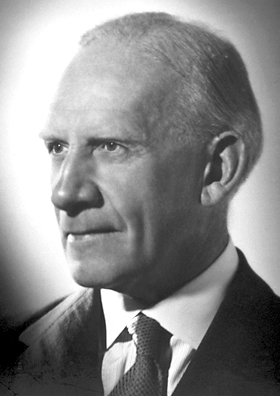
\includegraphics[width=\linewidth]{images/book3/robinson.jpg}
\end{minipage}\hfill
\begin{minipage}[t]{0.78\linewidth}
\vspace{0pt}
罗伯特·罗宾逊与威廉·拉普森于 1935 年发表了这一\omterm{def:b2:conjugate-additions:robinson}{成环反应}序列，其工作旨在
合成甾体。罗宾逊的主要成就是生物碱的结构与合成，
因此获 1947 年诺贝尔化学奖。1950 年，彼得·维兰德与卡尔·米舍尔制得
本章问题中的双环二酮，该物质此后成为甾体和
萜类合成的常用起点。（肖像：作者不详，公有领域；维基共享资源。）
\end{minipage}
\end{history}

\begin{safety}{\ghs[5mm]{GHS02}\,\ghs[5mm]{GHS05}\,\ghs[5mm]{GHS06}\,\ghs[5mm]{GHS07}\,\ghs[5mm]{GHS08}\,\ghs[5mm]{GHS09}}
丁-3-烯-2-酮易燃、剧毒、有腐蚀性，对水生环境有害，并为强催泪剂，仅
可在通风橱中操作。环己-2-烯-1-酮易燃且有毒。有机锂试剂、格氏试剂和
\omterm{def:b2:conjugate-additions:cuprate}{有机铜锂试剂}遇水剧烈反应，须在惰性气体下操作。
% ledger: ghs:MVK, ghs:cyclohexenone, ghs:MeMgBr
\end{safety}

\section{练习}

\begin{exercise}[$\star$]\label{exo:b2:conjugate-additions:1}
预测下列试剂与环己-2-烯-1-酮发生 \omterm{def:b2:conjugate-additions:addition-modes}{1,2-加成}还是 1,4-加成：\ce{CH3MgBr}；\ce{(CH3)2CuLi}；
\ce{C6H5SH}（加少量碱）；\ce{LiAlH4}。
\end{exercise}

\begin{exercise}[$\star$]\label{exo:b2:conjugate-additions:2}
将下列物质分类为\omterm{def:b2:conjugate-additions:michael}{迈克尔给体}或\omterm{def:b2:conjugate-additions:michael}{迈克尔受体}：戊-2,4-二酮、丙烯腈 \ce{CH2=CHCN}、
硝基甲烷、丙烯酸甲酯、丙二酸二乙酯、丁-3-烯-2-酮。
\end{exercise}

\begin{exercise}[$\star$]\label{exo:b2:conjugate-additions:3}
写出由 1-溴丁烷、锂和碘化亚铜制备二丁基铜锂的过程。
\end{exercise}

\begin{exercise}[$\star$]\label{exo:b2:conjugate-additions:4}
求丙二酸二乙酯与丁-3-烯-2-酮在催化量乙醇钠
存在下的产物，以及其水解并加热后的产物。
\end{exercise}

\begin{exercise}[$\star\star$]\label{exo:b2:conjugate-additions:5}
以环己-2-烯-1-酮为原料，提出 3-甲基环己酮的制备路线，并说明
为何溴化甲基镁不宜选用。
\end{exercise}

\begin{exercise}[$\star\star$]\label{exo:b2:conjugate-additions:6}
乙硫醇在痕量三乙胺存在下与丁-3-烯-2-酮发生加成。写出反应机理，并说明
硫醇负离子为何发生 1,4-加成。
\end{exercise}

\begin{exercise}[$\star\star$]\label{exo:b2:conjugate-additions:7}
氰离子与环己-2-烯-1-酮反应，低温、短时间下得到氰醇；
温度较高、时间较长时，则得到 3-氧代环己烷-1-甲腈。
试用动力学控制和热力学控制加以解释。
\end{exercise}

\begin{exercise}[$\star\star$]\label{exo:b2:conjugate-additions:8}
写出 2-甲基环己烷-1,3-二酮与丁-3-烯-2-酮的\omterm{def:b2:conjugate-additions:robinson}{罗宾逊成环}产物，然后
写出环己酮与丁-3-烯-2-酮的\omterm{def:b2:conjugate-additions:robinson}{罗宾逊成环}产物。
\end{exercise}

\begin{exercise}[$\star\star$]\label{exo:b2:conjugate-additions:9}
将庚烷-2,6-二酮切断为一个\omterm{def:b2:conjugate-additions:michael}{迈克尔给体}和一个\omterm{def:b2:conjugate-additions:michael}{迈克尔受体}，并提出反应条件。
\end{exercise}

\begin{exercise}[$\star\star\star$]\label{exo:b2:conjugate-additions:10}
简单的\omterm{def:b2:enolates-aldol:aldol}{羟醛加成}在碱性条件下易于逆转，而丙二酸二乙酯与
丁-3-烯-2-酮的\omterm{def:b2:conjugate-additions:michael}{迈克尔加成}产物则不然。试从形成和断裂的化学键以及产物的酸性加以解释。
\end{exercise}

\begin{exercise}[$\star\star\star$]\label{exo:b2:conjugate-additions:11}
丙二酸二乙酯与两当量丙烯酸甲酯在催化量碱存在下反应，得到一种产物，
其两个酯基之间不再含有 \ce{C-H}。画出该产物并加以解释。
\end{exercise}

\begin{exercise}[$\star\star\star$]\label{exo:b2:conjugate-additions:12}
2-甲基环己酮与丁-3-烯-2-酮进行\omterm{def:b2:conjugate-additions:robinson}{罗宾逊成环}反应时，可经任一\omterm{def:b2:enolates-aldol:enolate}{烯醇负离子}反应。
画出两种产物，并说明哪些条件有利于甲基位于环稠合
碳上的那一种生成。
\end{exercise}

\section{问题：维兰德–米舍尔酮}

\begin{problem}[{周末问题——酸性给体、迈克尔加成产物、分子内羟醛缩合
及其脱水、手性碳原子与制备的质量衡算}]
\label{pb:b2:conjugate-additions:1}
制备（练习数据）：取 \qty{10.0}{g} 2-甲基环己烷-1,3-二酮，与略过量的
丁-3-烯-2-酮及催化量的碱发生反应（\omterm{def:b2:conjugate-additions:michael}{迈克尔加成}）；随后该三酮与
\omterm{def:b2:amines:class}{仲胺}和酸发生环化（\omterm{def:b2:enolates-aldol:aldol}{羟醛缩合}、脱水）。总产率为 70~\%。母体环己烷-1,3-二酮在水中的
$\mathrm pK_a = 5.3$。摩尔质量（\unit{g/mol}）：C 12.011，H 1.008，O 15.999。
% ledger: pka:cyclohexanedione, aw:C, aw:H, aw:O, ghs:methylcyclohexanedione, ghs:MVK

\medskip
\noindent\textbf{第一部分——给体。}
\begin{enumerate}
  \item 画出 2-甲基环己烷-1,3-二酮，并标出其酸性最强的氢。
  \item 为何该氢的酸性远强于环己酮的 $\alpha$ 氢？
  \item 画出其\omterm{def:b2:enolates-aldol:enolate}{烯醇负离子}的三种共振结构。
  \item 氢氧根或乙氧根是否足以完全生成该\omterm{def:b2:enolates-aldol:enolate}{烯醇负离子}？请利用 $\mathrm pK_a$ 判断。
  \item 写出涉及 C2 的二酮的\omterm{def:b2:enolates-aldol:tautomerism}{烯醇}式，并说明 C2 上的甲基
        为何不妨碍其生成。
  \item 它是\omterm{def:b2:frontier-orbitals:hard-soft}{硬亲核试剂}还是\omterm{def:b2:frontier-orbitals:hard-soft}{软亲核试剂}？它会进攻丁-3-烯-2-酮的哪一个位点？
\end{enumerate}

\medskip
\noindent\textbf{第二部分——\omterm{def:b2:conjugate-additions:michael}{迈克尔加成}产物。}
\begin{enumerate}[resume]
  \item 写出\omterm{def:b2:conjugate-additions:michael}{迈克尔加成}反应，并命名生成的三酮。
  \item 为何只需催化量的碱？
  \item 为何新键生成于二酮的 C2 而非氧原子上？
  \item 该三酮中含有几个季碳？
  \item 指出该三酮中的 1,5-二羰基关系。
  \item 为何使用略过量的丁-3-烯-2-酮，且只能略过量？
\end{enumerate}

\medskip
\noindent\textbf{第三部分——成环。}
\begin{enumerate}[resume]
  \item 列出三酮中带有 $\alpha$ 氢的碳原子。
  \item 哪种\omterm{def:b2:enolates-aldol:enolate}{烯醇负离子}进攻哪一个羰基，可形成六元环？
  \item 还可尝试哪些其他的成环方式？为何它们不能得到目标产物？
  \item 写出生成的\omterm{def:b2:enolates-aldol:aldol}{羟醛}产物及随后的脱水反应。
  \item 为何脱水反应容易进行？
  \item 命名维兰德–米舍尔酮所含的官能团。
\end{enumerate}

\medskip
\noindent\textbf{第四部分——立体化学与质量衡算。}
\begin{enumerate}[resume]
  \item 产物中哪一个碳原子是手性碳原子？
  \item 该制备所得产物是否具有旋光性？请说明理由。
  \item 计算二酮、丁-3-烯-2-酮及产物
        \ce{C11H14O2} 的摩尔质量。
  \item 写出总反应方程式，并据化学式进行核对。
  \item 计算所用二酮的物质的量。
  \item 说明在总产率为 70~\% 时所得维兰德–米舍尔酮的质量。
\end{enumerate}
\end{problem}
